\section{Discussion}\label{discussion}

\subsection{Time Evolution}\label{discussion:normal}

In Sect.~\ref{results_normal} we have seen that the shape of VSFs measured for the gas of simulated molecular clouds evolves in the same way as the clouds themselves.
For example, Fig.~\ref{pic:results:zeta_all}a demonstrates that the measured $\zeta$ cease with time as the clouds contract under the influence of self-gravity.
This is evident as the density and boundness of the clouds increases \textbf{as} further gas falls into them \citepalias{IbanezMejia2017}.

However, one also sees peaks in the profiles of $\zeta$ that represent a temporary deviation from the global evolution of the clouds.
The origin of these features can easily be traced back to the SNe occurring in the environment of the clouds.
To visualise this better, we add marks to Fig.~\ref{pic:results:zeta_all} that represent the times when the SNe explode and the periods of time when the clouds are heavily accreting gas.
The data are taken from \citetalias{IbanezMejia2017}, where mean distances between the sites of SNe and the centres of the clouds can also be found.
Considering that the SNe shock fronts move at speeds of 50--100~km~s$^{-1}$ through the ISM and with distances between 30--100~pc to the clouds, the shocks need around 1~Myr, on average, to reach the clouds.
Thus, one cannot only relate the major gas accretion events of the clouds to the arrival of those SNe, that indeed affect the evolution of the clouds, but also all significant variations in the evolution of $\zeta$.
In most of the cases, the SNe inject turbulent power into the systems.
This amplifies the VSFs at all scales, but in particular the large scales, causing an elevation of $\zeta$.
However, the interaction between the clouds and the shocks lasts only for less than 0.6~Myr, after which $\zeta$ evolves back into the pre-shock conditions

The behaviour of \texttt{M8} appears to contradict the \textbf{above explanations which we explain as follows}:
In the beginning, \texttt{M8} evolves only slightly.
It loses a small fraction of gas \citepalias[Fig.~5, \textit{middle} panel]{IbanezMejia2017}.
Therefore, the VSFs increase towards larger separations.
At $t$~=~1.5~Myr the shock front of the $t$~=~0.8~Myr SN hits the cloud.
That causes a short period of extreme gravitational collapse, traced by the dip in $\zeta$.
As in the other clouds, the gas relaxes rapidly after the shock.
However, the interaction with the shock the cloud has introduced instability into the clouds that continues to gravitationally contract.
That is seen as slow decrease of $\zeta$ from $t$~=~1.8~Myr on. 

In summary, one can say that the scaling exponent, $\zeta$, that is obtained by fitting a power-law relation onto the measured VSF, is a useful tool to understand and evaluate the time evolution of turbulence within molecular clouds. 
It is not only sensitive to both external (SNe) and internal (gravitational collapse) driving sources, but also reacts differently to the individual driving sources. 

However, this diagnostic requires a series of time steps to be significant.
According to \citet{She1994} and \citet{Boldyrev2002}, $\zeta$(3) is supposed to be equal or larger than unity whenever the gas experiences supersonic turbulence.
Although this is definitely the case in the simulated clouds \citepalias{IbanezMejia2016,IbanezMejia2017}, one sees that $\zeta$(3) declines far below 1 due to gravitational collapse.
Thus, measuring $\zeta$ for individual moments in time, as observations would do, cannot fully describe the turbulence of molecular clouds.

The principle of "extended self-similarity" \citep[Sect.~\ref{methods:vsf}]{Benzi1993} offers a solution to this problem.
The principle reflects the nature and the properties of intercloud turbulence, even when it is dominated by gravitational collapse.
However, we also detect strong deviations that either reduce or increase the measured values of $Z$ (see Fig.~\ref{pic:results:z_all}a).
Those derivations can be related to the physical forces that currently dominate the clouds.

The peaks in the $Z$ (for example, in \texttt{M4} at $t$~=~4.1~Myr) occur at the times when the respective $\zeta(3)$ reaches values close or below 0.
This means that the VSF becomes flat ($\zeta$~=~0) or increases forward smaller scales ($\zeta~<~0$). 
In this case, self-gravitational contraction clearly dominates the cloud's evolution as it transfers turbulent power from the large to the small scales, where filaments and fragments are forming and accreting gas.

The decrease in $Z$ (for example, in \texttt{M3} around $t$~=~1.8~Myr), on the other hand, occur when SN shocks hit and heavily impact the clouds. 
This causes a sudden, but heavy increase of turbulent power on all scales, though on the larger scales more than on the smaller, resulting in a steepening of the VSF towards larger scales and an increase in $\zeta$.
The VSFs become more sensitive to the shock the higher their order is.
Therefore, the $\zeta(3)$ increases more rapidly than $\zeta(2)$ and $\zeta(1)$, causing $Z(2)$ and $Z(1)$ to decrease.

In summary, $Z$ \textbf{is only a weak tracer for gravitational contraction, but a good tracer for shocks interacting with the cloud.}
Whenever neither of these two extreme scenarios is acting on the clouds, the values of $Z$ are close to the predicted values (see discussion below).
This means that \textbf{$Z$ and $\zeta$ are good tracers for processes suddenly driving turbulence within the cloud.
However, when Z values are close to the ones predicted by theory, we cannot differentiate between freely decaying turbulence and moderate gravitational contraction}, as one can do it with $\zeta$.
However, the advantage is that a single-epoch observation of $Z$ is sufficient to trace extreme motions and driving sources within observed molecular clouds.

Whenever the turbulence within the clouds is not driven in an extreme way one sees that the ratio of the VSF scaling exponents is mostly in agreement with predicted values for self-similar turbulence, although the clouds are dominated by gravitationally contracting motions during their evolution.
\textbf{The measured values of $Z$} do not uniquely follow the predictions of only \citet{Boldyrev2002} or \citet{She1994}, but are normally between the predicted values.
Recalling that both studies describe supersonic, fully developed turbulent flows, the only difference between them is the geometry along which they allow the gas to flow.
In the case of \citet{Boldyrev2002}, the gas flows are sheet-like, while they are filamentary in the work by \citet{She1994}.

Since \texttt{M3} is heavily impacted by many SN shocks and strong collapsing motions, it does not allow us to make strong predictions about its 'steady-state' evolution.
The other two clouds, on the contrary, are less externally impacted.
This allows us to relate the developments of measured $Z$ to the internal evolution of the clouds.
In \texttt{M8}, $Z$ follows the predictions by \citet{She1994} for most of the time.
This \textbf{would suggest} that \texttt{M8} mostly transfers gas along filamentary substructures which means that the cloud is highly hierarchically structured already at the beginning of the simulations and before self-gravity is active.
This also implies that the formation of filamentary structures does not require gravity \citep[e.g.,][]{Federrath2016}.
The fact that we do not detect fragments before the clouds have evolved under the influence of self-gravity for at least one megayear \citepalias[see][]{Chira2018}, however, demonstrates that gravity is essential for the fragmentation of filaments and formation of further substructures.

The evolution of $Z$ in \texttt{M4} shows a slightly different picture.
While the values of $Z$ in \texttt{M8} are mostly constant over time, they decrease in \texttt{M4}, starting at values that are in agreement with the sheet-like flows of \citet{Boldyrev2002} to those that are predicted for filamentary flows by \citet{She1994}. 
This demonstrates that \texttt{M4} develops its hierarchical structure as it evolves under the influence of self-gravity. 
As a consequence, its turbulent structure becomes more dominated by the filaments with time which causes the decline of $Z$.
Considering that the gas of \texttt{M4} is indeed first flattened into more sheet-like geometry through the impact of the SNe \citepalias{IbanezMejia2017} this observation is very interesting.
It agrees with the studies, for example by \citet{Lin1965} or \citet{McKee2007}, that claim that molecular clouds are supposed to collapse in a dimension-losing, outside-in fashion that does not require any initial substructures within the clouds.

In summary, $Z$ reflects the global geometry of turbulence within molecular clouds. 
Thereby, the measured values of $Z$ are in good agreement with predictions from self-similarity theory, as long as one carefully ensures that the dominating turbulence mode in the cloud matches the modes that are considered in the respective theory.
This makes $Z$ a reliable parameter for examining turbulence modes in observational studies.
Furthermore, the time evolution of $Z$ shows how the geometry of turbulence is changed due to the gravitational contraction, e.g.~from sheet-like to filamentary vortices, accompanies the change of basic parameters describing the turbulent structure of the entire cloud. 
$Z$ can also deviate from the predicted values. 
This, however, only occurs in time spans of extreme turbulence driving, such as SN shocks.
Thereby, these extreme driving sources affect $Z$ differently:
SN shocks decrease $Z$, while gravity causes a \textbf{short-lived} peak in $Z$.
In both cases, $Z$ relaxes to the pre-perturbation values within a short time.




\subsection{Comparison to Line-of-Sight Velocities}\label{discussion:1d}

In this paper, we do not only aim to analyse the mechanisms that drive turbulence within simulated molecular clouds, but also to provide a practical tool that can be used to understand the dynamical processes within the ISM better.
For the latter, it is necessary to examine its applicability under and the dependencies of the obtained results on all relevant conditions. 
As we have chosen to use VSFs for our analysis it is evident that we first need to investigate how the function reacts to the number of measured velocity vector components. 

We recall that the VSF relates to the average relative velocity between the clouds' gas cells (see Eq.~(\ref{equ:method:def_vsf})).
This means that for a proper analysis one needs all three components of the three-dimensional (3D) velocity vector for each contributing cell.
Observations, however, normally measure only the one (1D) component along the line-of-sight (los), also known as local standard of rest velocity.
If the gas moves exclusively along the los, both the 3D and 1D velocity measurements will return the same VSF. 
If the gas is, contrary, moving along directions perpendicular to the los the 1D VSF will be absolutely 0.
 
In this section, we discuss the results considering this aspect.
Hence, we use the same data of the model clouds as before and produce three subsamples by projecting the 3D velocity vectors onto the three major axes x, y, and~z, respectively.
The derived $\zeta$ and $Z$ for each subsample are shown in Figs.~\ref{pic:results:zeta_all}b and~\ref{pic:results:z_all}b.

In Sect.~\ref{results:1d} we have seen that the $\zeta$ and $Z$ derived from the 1D VSFs generally evolve similarly as those derived from the 3D VSFs.
Yet, we have also seen that individual sight lines may evolve differently.
Those differences are generated when the gas is significantly more driven into the corresponding los than into the others (analogously to the simple scenario described above). 

For example, for the first two megayears of the evolution of \texttt{M4} the values of $Z$ along the y axis are significantly higher than those observed along the other axes and the predicted values.
Recalling that a higher value of $Z$ correspond to an episode of very strong gravitational contraction, we can conclude that within this time span \texttt{M4} is dominantly collapsing along its y axis. 
The values of $Z$ that are measured for the other two axes agree with this conclusion as they are best predicted by \citet{Boldyrev2002} who describes a sheet-like turbulence. 
Note that this effect is only visible as we analyse the three dimensions separately, while the driving of the gas along the y axis is averaged out in the 3D VSFs (see Fig.~\ref{pic:results:z_all}a).

In summary, we see that for a fully developed 3D turbulent field we expect that 1D VSFs behave similarly to 3D VSFs.
However, when there is a preferred direction along which the gas flows the 1D and 3D VSFs differ significantly from each other. 
Thus, we predict that observed VSFs reflect the nature of turbulence within molecular clouds unless there is clear evidence that the gas is driven into a particular direction (e.g., by an proto-/stellar feedback, or SN shock front).

Note that in this analysis does not take typical los effects, such as optical depth effects or blending, into account. 
As we have seen in Sect.~\ref{results:densthres}, a good knowledge of the origin of velocity information is essential for a proper interpretation of the obtained VSFs.
Future studies need to investigate this point in more detail by performing elaborated radiative transfer calculations. 



\subsection{The Effect of Density Thresholds}\label{discussion:densthres}

\textbf{In Sect.~\ref{results:densthres} we have tested the influence of the density threshold that defines the volume of interest on the behaviour of the VSF.
In the work presented in this paper, we normally define the clouds as volumes of connected gas cells with number densities above n$_\mathrm{cloud}$~=~100~cm$^{-3}$.
Although this approach is in agreement with typical post-processing methods of observational data, it also means that we analyse only $\leq$1.5\% of the cubes' volumes, ignoring the more diffuse parts at the outer rims of the molecular clouds and the ISM.
This raises the question: Are the turbulent motions within the entire ISM and the denser molecular clouds driven by the same processes?
For targeting this question we have repleated our analysis and set n$_\mathrm{cloud}$~=~0~cm$^{-3}$.
Figs.~\ref{pic:results:zeta_all}c and~\ref{pic:results:z_all}c illustrate the results.
}

We see that the structure and behaviour of VSFs strongly depends on whether or not there is a density threshold. 
In the previous case, where n$_\mathrm{cloud}$~=~100~cm$^{-3}$, we have seen a mostly straight decline of $\zeta$ and a rather constant evolution of $Z$ over time that reflect the contraction of the clouds due to self-gravity.

Here, in the n$_\mathrm{cloud}$~=~0~cm$^{-3}$ sample, we observe a completely different picture.
There is still a slightly declining trend in $\zeta$, yet the evolutions are dominated by random fluctuations.
We also see that the measured $Z$ evolves completely constantly.
This is true for the entire time range and the exactly same values of $Z$ measured for all clouds.
This can only be the case when the here analysed VSFs reflect the turbulent structure of the entire ISM in which all three clouds are embedded in.
Furthermore, the source that drives the turbulence within the ISM acts constantly and isotropically on the diffuse gas.
Thus, the ISM matter around the clouds can not be driven by individual events, like single SNe, as they do not have a high enough impact on the entire ISM, particularly not compared to the impact they have on individual molecular clouds that are comparably quiet zones within the ISM.

We conclude that the decision whether or not a density threshold is used for ascertaining insights on the turbulent composition of the observed gas has a significant and direct influence on the resulting VSFs.
However, as mentioned previously, applying a density threshold is often unavoidable as it is a straight-forward approach to filter the data on the actual area of interest.
In observational studies it is even always present as minimal collision rates for excitation or the sensitivity of detectors automatically introduce an implicit density or intensity thresholds. 
Although we have only tested two specific setups in this context we have seen the significance of a proper choice of the density threshold, as well as a proper discussion of the obtained results considering the used threshold as one of the defining parameters.



\subsection{The Effect of Density Weighting}\label{discussion:densweight}

In this subsection, we discuss the effect the ambiguous definition of VSFs has on the measurements. 
With this we mean that the VSF can be computed with or without taking density weighting into account.
This ambiguity originates in the type of data one analyses.
In general, the VSF considers the average relative velocity between two individual Lagrangian particles or turbulent vortices.
As each particle stores its complete set of information, its mass, and therefore its inertia, is automatically considered when iterating its velocity.
This makes Eq.~(\ref{equ:results:def_vsf_no}) sufficient for deriving the VSF of the fluid properly.

In our case, however, we examine Eulerian data that store the parameters of the fluid on a static grid. 
The information of individual particles and vortices are, thereby, averaged over the grid.
Consequently, it is important to consider this when computing the VSF.
This is done by using the density-weighted definition of the VSF given in Eq.~(\ref{equ:method:def_vsf}).

Although the motivation why there are different definitions of the VSF and why they are used for non-overlapping samples of data, it is not yet clear how the results obtained with the two approaches relate to each other. 
We investigate that question by applying both approaches on our data.
The results are presented in Sect.~\ref{results:densweight}.

We see that, as long as the turbulence is dominated by the large scales, considering the density weighting or not does not have a significant effect on the data. 
However, as the clouds evolve the differences increase because the non-weighted VSFs never drop below 0.5.
This is because the non-weighted VSF treats all cells equally, no matter whether the particular cell represents a dense element of the cloud centre or a diffuse element of the cloud's edge, while the weighted VSF gives more weight to the matter within the clouds.
As long as the turbulence is dominated by large scales this does not cause a notable difference as these long separations represent cells on the outer surface of the clouds, with similar densities and conditions.
The small lag scales, contrary, reflect how the conditions change within the clouds, with density gradients becoming larger towards the centre of the clouds and increasing faster than the relative velocities of neighbouring cells.
In this case, the density weighting becomes crucial to compensate for the fact that the higher density represents a higher number of particles in a Lagrangian framework.
However, if one does not consider this (as we do when using the non-weighted definition of the VSF) the inner regions of the clouds are not processed correctly.
This ends in a situation where the large scales never seem to loose their dominance in term of kinetic energy, and $\zeta$ never becomes close or less than 0; a situation that does not reflect the reality.

In summary, we can trace the discrepancies between the scaling exponents of density-weighted and non-weighted VSFs back to the \textbf{inability} of the non-weighted VSFs to follow the transition form large-scale driven to small-scale dominated distributions of turbulent power.


Nevertheless, Fig.~\ref{pic:results:z_all}d illustrates that these differences can be traced by $\zeta$ only. 
Besides the features created when $\zeta$ becomes close to 0 in the density-weighted VSFs, the measured $Z$ have similar values, evolve and reacts to external driving mechanisms similarly independently based on which approach they are computed. 
This observation is true for all Jeans refinement levels, as Fig.~\ref{pic:results:comp_weighting} demonstrates.

We conclude that deriving the VSF from smooth density distributions without considering density weighting does not affect the behaviour of $\zeta$ and $Z$, as long as the turbulence is dominated by large scale vortices, while it has a significant effect on the measurements when the small scales become dominant.
The latter is particularly important as this finding has a directly impact on the conclusions drawn based on the scales and mechanisms that drive the turbulence based on the measured $\zeta$.
Not only does $\zeta$ become insensitive from the influence of gravitational contraction with time, the non-weighted VSFs do also not reflect when the majority of kinetic energy has been transferred to small scales. 
Thus, it is highly important to clarify which definition of VSF is used and if it is indeed suitable for the respective study.
Yet, our analysis also shows that the principle of self-similarity relativises the deviations between the two approaches as the different orders of the VSFs keep scaling in the same way relative to each other. 




\subsection{The Effect of Jeans Length Refinement}\label{discussion:refinement}

In Sect.~\ref{results:refinement}, we have motivated the need to investigate the influence of Jeans refinement on VSFs.
In particular, we examine how the choice of using the minimal required refinement compares to a generally recommended refinement level, including the differences in total energy and resonances seen in the power spectra. 
To do this, we use the data by \citetalias{IbanezMejia2017} that resolve the Jeans length in \texttt{M3} twice ($\lambda_J$~=~$8\Delta{}x$) and eight times ($\lambda_J$~=~$32\Delta{}x$) finer as the original simulations ($\lambda_J$~=~$4\Delta{}x$).

In Fig.~\ref{pic:results:jeans_comp} we see that the choice of refinement level does not have to have a significant influence on the measurements and evolution of both $\zeta$ and $Z$. 
$\lambda_J$~=~$4\Delta{}x$ and $\lambda_J$~=~$8\Delta{}x$ are in very good agreement with each other.
This means that, although refining Jeans lengths with 4~cells misses about 13\% of kinetic energy, the effect on the structure and behaviour of the turbulence is rather small and not traced by the VSF analysis.

However, Fig.~\ref{pic:results:jeans_comp} shows that such an agreement is not given with $\lambda_J$~=~$32\Delta{}x$, as latter differs more from $\lambda_J$~=~$4\Delta{}x$ the higher the order of the VSF is.
Following the explanations in Sect.~\ref{results:refinement}, the behaviour of $\zeta$ and $Z$ in the $\lambda_J$~=~$32\Delta{}x$ runs corresponds to the reaction of the cloud's gas to a shock wave running through the cloud; caused by a supernova that exploded before $t$~=~0~Myr. 
Indeed one sees a SN at a distance of 172~pc at $t$~=~-1.11~Myr. 
Due to the distance the SN is too weak to effectively compress the gas within \texttt{M3} and causing a shock.
This is why it has not been detected previously in the less refined samples.
However, the SN explodes far below the mid-plane of the simulated disk galaxy, in a region without dense gas.
This means that the shock wave, that has been injected by the explosion, is less damped as it propagates through the ISM. 
By the time the front arrives at \texttt{M3} it is still energetic enough to drive strong winds, with velocities above 300~km~s$^{-1}$, at the closer edge of the cloud. 
This causes an increase of VSFs at longer lag scales and the increase of $\zeta$, as well as the drop in $Z$.

Derivations of measured $Z$ to predicted values do trace external turbulent driving.
Whether the source is a SN shock front propagating through the cloud or a strong wind, cannot be distinguished by $Z$ only. 
Yet, $Z$ remains a fine probe for the geometry of turbulence and the scales at which turbulence is driven.


\subsection{Comparison to Observational Data}\label{discussion:observation}

\rc{[completely new]}

%mm [removed use of multirow and excess lines to stay within standard A&A style]
\begin{table*} 
\centering 
	\begin{tabular}
%mm {l|l|ccc}
        {llccc} 
	\centering 
		Reference & Comments & p & $\zeta$ & Z \\ \hline  \hline
		
%mm \multirow{2}{*}{ }
\citet{Heyer2004} & $^{12}$CO J = 1-0, & 
               %mm \multirow{2}{*}{
                   1 &  
              %mm \multirow{2}{*}{
                     0.49 $\pm$  0.15 &  
                             %mm \multirow{2}{*}{
                                          0.49 $\pm$  0.15 \\ 
					& Perseus \& Solar Neighborhood & & & \\ \hline
%mm \multirow{2}{*}{
             \citet{Heyer2015} & $^{12}$CO \& $^{13}$CO J = 1-0, 30 MCs & 1 &  0.24 $\pm$  0.00 &  0.24 $\pm$  0.00 \\ 
					 & $^{12}$CO \& $^{13}$CO J = 1-0, Taurus & 1 &  0.26 $\pm$  0.00 &  0.26 $\pm$  0.00 \\  \hline
%mm \multirow{2}{*}{
           \citet{Miesch1994} & $^{13}$CO J = 1-0, & 1 &  0.43 $\pm$  0.15 &  0.43 $\pm$  0.15 \\ 
					   & 12 clouds and subregions of GMCs & 2 &  0.86 $\pm$  0.30 &  0.86 $\pm$  0.30 \\  \hline
%mm \multirow{6}{*}{
     \citet{Padoan2003} & 
     %mm \multirow{3}{*}{
         $^{13}$CO J = 1-0, Perseus & 1 &  0.50 $\pm$  0.00 &  0.42 $\pm$  0.00 \\ 
					   &  & 2 &  0.83 $\pm$  0.00 &  0.72 $\pm$  0.00 \\ 
					   &		 & 3 &  1.18 $\pm$  0.00 &  1.00 $\pm$  0.00 \\ 
					  & 
       %mm \multirow{3}{*}{
              $^{13}$CO J = 1-0, Taurus & 1 &  0.46 $\pm$  0.00 &  0.42 $\pm$  0.00 \\ 
					   &		 & 2 &  0.77 $\pm$  0.00 &  0.72 $\pm$  0.00 \\ 
					   &		 & 3 &  1.10 $\pm$  0.00 &  1.00 $\pm$  0.00 \\  \hline
		\citet{Padoan2006} & $^{13}$CO J = 1-0, Perseus & 2 &  0.80 $\pm$  0.10 &  0.80 $\pm$  0.10 \\  \hline
		\citet{RomanDuval2011} & $^{13}$CO J = 1-0, 367 clouds from the GRS survey & 1 &  0.50 $\pm$  0.30 &  0.50 $\pm$  0.30 \\  \hline
%mm \multirow{4}{*}{
\citet{Zernickel2015} & 
         %mm \multirow{2}{*}{
                   $^{13}$CO J = 1-0, NGC 6334 & 1 &  0.38 $\pm$  0.00 &  0.38 $\pm$  0.00 \\ 
					   &		 & 2 &  0.76 $\pm$  0.01 &  0.76 $\pm$  0.01 \\ 
					 & 
                 %mm \multirow{2}{*}{
                      $^{13}$CO J = 1-0, NGC 6334, $\ell \leq$ 4 pc  & 1 &  0.48 $\pm$  0.01 &  0.48 $\pm$  0.01 \\ 
					   & & 2 &  0.79 $\pm$  0.01 &  0.79 $\pm$  0.01 
	\end{tabular} 
	\caption{Summary of observed $\zeta$ and Z in the literature.} 
	\label{tab:discussion:summary_obs} 
\end{table*} 


\begin{figure*}
	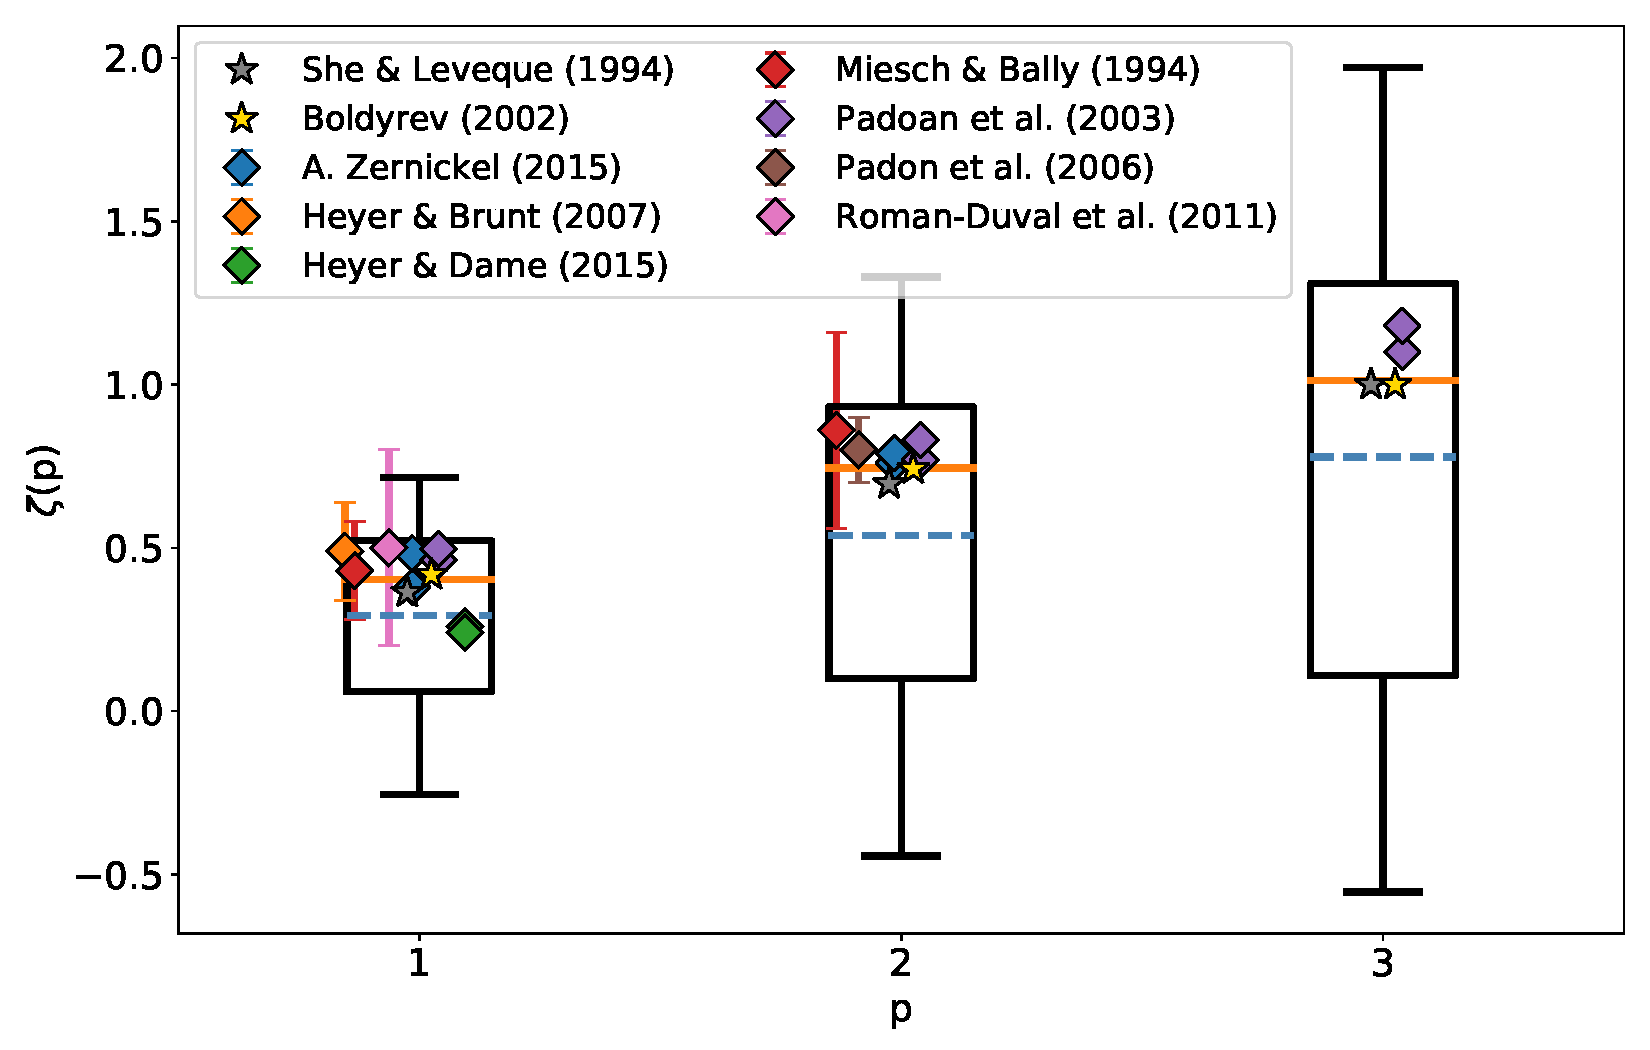
\includegraphics[width=\textwidth]{compare_observations.pdf}
	\caption{Summary of measurements of $\zeta$ (\textit{abscissas}) and $Z$ (\textit{ordinates}) for orders $p$~=~1--3 (from \textit{left} to \textit{right}) in this study and in the literature.
		The grey markers represent the values as presented in Sect.~\ref{results:normal}, while the coloured star markers illustrate the predictions by \citet{She1994} and \citet{Boldyrev2002}. The coloured, circular marker summarise values found in the literature (see legend for precise references). 
	}
	\label{pic:discussion:comp_observation}
\end{figure*}











